\documentclass[10pt,a4paper]{book}
\usepackage[utf8]{inputenc}
\usepackage[spanish]{babel}
\usepackage{amsmath}
\usepackage{amsfonts}
\usepackage{amssymb}
\usepackage{makeidx}
\usepackage{graphicx}
\usepackage{multicol}
\begin{document}
\begin{center}
\textbf{CAPÍTULO III}
\end{center}
\section{ DERIVADAS DE FUNCIONES}
La derivada de una función compleja de una Variable Compleja se define, exactamente, de la misma manera que el caso real del cálculo elemental.
\\
\\
\subsection{DEFINICIÓN}
Sea $f:D \subset C \rightarrow C$, una función compleja de variable compleja, entonces la derivada $f'$ de la función $f$ en el punto $z_0$ está dado por:\\
$$f'(z_0)= \lim\limits_{\ \vartriangle z \rightarrow 0}\frac{f(z_0+\vartriangle z)-f(z_0)}{\vartriangle z}$$
\\
siempre y cuando el límite exista.
\subsection{PROPIEDADES DE LA DERIVADA DE FUNCIONES COMPLEJAS}
Sean $f,g:D \subset C \rightarrow C$ funciones complejas y $k$ una constante compleja entonces:
\\
\\
1.- Si $w=f(z)=k \qquad \Rightarrow \frac{dw}{dz}=0$
\\
\\
2.- Si $w=k f(z) \qquad \Rightarrow \frac{dw}{dz}=k.f'(z)$
\\
\\
3.- Si $w=f(z)\pm g(z) \qquad \Rightarrow \frac{dw}{dz}=f'(z)\pm g'(z)$
\\
\\
4.- Si $w=(f.g)(z) \qquad \Rightarrow \frac{dw}{dz}=f'(z).g(z)+f(z).g'(z)$
\\
\\
5.- Si $w=\frac{(f)(z)}{g(z)} \qquad \Rightarrow \frac{dw}{dz}=\frac{g(z).f'(z)-f(z).g'(z)}{g^{2}(z)},  g(z)\neq0$
\\
\\
La demostración de estas propiedades son idénticas al de las funciones reales del cálculo elemental, demostraremos la propiedad $(4)$.
\\
\\
$\frac{dw}{dz}= \lim\limits_{\ \vartriangle z \rightarrow 0}\frac{f(z+\vartriangle z).g(z+\vartriangle z)-f(z).g(z)}{\vartriangle z}$
\\
\\
\\
$\frac{dw}{dz}= \lim\limits_{\ \vartriangle z \rightarrow 0}\frac{f(z+\vartriangle z).g(z+\vartriangle z)-f(z+\vartriangle z).g(z)+f(z+\vartriangle z).g(z)-f(z).g(z)}{\vartriangle z}$
\\
\\
\\
$\frac{dw}{dz}= \lim\limits_{\ \vartriangle z \rightarrow 0} \lbrace f(z+\vartriangle z).[\frac{g(z+\vartriangle z)-g(z)}{\vartriangle z}]+g(z).[\frac{f(z+\vartriangle z)-f(z)}{\vartriangle z}]\rbrace$
\\
\\
\\
$\frac{dw}{dz}=f(z) \lim\limits_{\ \vartriangle z \rightarrow 0} \frac{g(z+\vartriangle z)-g(z)}{\vartriangle z} +g(z)\lim\limits_{\ \vartriangle z \rightarrow 0} \frac{f(z+\vartriangle z)-f(z)}{\vartriangle z}$
\\
\\
\\
$\frac{dw}{dz}=f(z).g'(z)+g(z).f'(z)$
\subsection{DEFINICIÓN}
La función $f:D \subset C \rightarrow C$ es derivable en el punto $z_0 \in  D$, si existe la derivada en $z_0 (f'(z_0))$ es decir:
\\
$$f'(z_0)= \lim\limits_{\ \vartriangle z \rightarrow 0}\frac{f(z_0+\vartriangle z)-f(z_0)}{\vartriangle z}$$
\\ 
Lo que es equivalente a:
\\
$$f'(z_0)= \lim\limits_{\ z \rightarrow z_0}\frac{f(z)-f(z_0)}{z-z_0}$$
\\
donde $\vartriangle z=z-z_0$ entonces $z=z_0+\vartriangle z$
\\
\\
además si $\vartriangle z \rightarrow 0$ entonces $z-z_0 \rightarrow 0$
\\
\\
de donde $z \rightarrow z_0$
\\
\\
$\vartriangle z=z-z_0=(x+iy)-(x_0+iy)=(x-x_0)+(y-y_0)i=\vartriangle x +i\vartriangle y$
\\
$$ \vartriangle z=\vartriangle x+i\vartriangle y$$
\\
$\vartriangle z \rightarrow 0$, entonces $\vartriangle x+i\vartriangle y \rightarrow 0$
\\
\\
de donde $\vartriangle x \rightarrow 0 \qquad \wedge \qquad \vartriangle y \rightarrow 0$
\\
\\
por lo tanto: $(\vartriangle x,\vartriangle y)\rightarrow (0,0)$
\subsection{3.4. INTERPRETACIÓN GEOMÉTRICA DE LA DERIVADA.-}
Sea $f:D \subset C \rightarrow C$ una función compleja y $z_0 \in D$ un punto $P$ en el plano complejo $(z)$ y sea $w_0$ su imagen $P'$ en el plano $(w)$ bajo la transformación $w=f(z)$, puesto que se supone que $f(z)$ es univoca, el punto $z_0$ es aplicado sólo en el punto $w_0$.
\\
\\
GRAFICO 1 Y GRAFICO 2
\\
\\
Al incrementar a $z_0$ en $\vartriangle z$ se obtiene el punto $Q$ este punto tiene como imagen a $Q'$ en el plano $(w)$, entonces se observa que $P'Q'$ representa al número complejo $\vartriangle w=f(z_0+\vartriangle z)-f(z_0)$, se reduce que la derivada en $z$ existe y está dado por:
\\
$$\lim\limits_{\ \vartriangle z \rightarrow 0}\frac{f(z_0+\vartriangle x)-f(z_0)}{\vartriangle z}=\lim\limits_{\ Q \rightarrow P}\frac{Q'P'}{QP}$$
\subsection{ECUACIONES DE CAUCHY-RIEMANN.-}
Se trata de obtener un par de ecuaciones que deben satisfacer las primeras derivadas parciales de las funciones componentes $u$ y $v$ de una función $f(z)=u(x,y)+iv(x,y)$ en un punto $z_0=(x_0,y_0)$ para que exista en el, la derivada de $f$, así mismo veremos como expresar $f'(z_0)$ en términos de tales derivadas parciales.
\\
\\
Suponiendo que $\exists f'(z_0)=\lim\limits_{\ \vartriangle z \rightarrow (0,0)}\frac{f(z_0+\vartriangle z)-f(z_0)}{\vartriangle z}$, sea $z_0=x_0+iy_0$ y $\vartriangle z=\vartriangle x+i\vartriangle y$, entonces por el teorema de límite se tiene:
\\
$$Re(f'(z_0))=\lim\limits_{\ (\vartriangle x,\vartriangle y) \rightarrow 0}Re(\frac{f(z_0+\vartriangle z)-f(z_0)}{\vartriangle z}) \textbf{...(1)}$$ 
\\
$$Im(f'(z_0))=\lim\limits_{\ (\vartriangle x,\vartriangle y) \rightarrow (0,0)}Im(\frac{f(z_0+\vartriangle z)-f(z_0)}{\vartriangle z}) \textbf{...(2})$$ 
\\
ahora agrupando se tiene:
\\
$$\frac{f(z_0+\vartriangle z)-f(z_0)}{\vartriangle z}=\frac{[u(x_0+\vartriangle x,y_0+\vartriangle y)-u(x_0,y_0)]+i[v(x_0+\vartriangle x,y_0+\vartriangle y)-v(x_0,y_0)]}{\vartriangle x+i\vartriangle y} \textbf{...(3)}$$
\\
Las expresiones $(1)$ y $(2)$ son variables cuando $(\vartriangle x,\vartriangle y) \longrightarrow (0,0)$ de todas las formas posibles, en particular es cuando $(\vartriangle x,\vartriangle y) \longrightarrow (0,0)$ horizontalmente por los puntos $(\vartriangle x,0)$.
\\
\\
GRAFICO
\\
\\
Quiere decir que $\vartriangle y=0$ en la ecuación $(3)$ resultan:
\\
\\
$Re(f'(z_0))=\lim\limits_{\ \vartriangle x \rightarrow 0}\frac{u(x_0+\vartriangle x,y_0)-u(x_0,y_0)}{\vartriangle x}$
\\
\\
$Im(f'(z_0))=\lim\limits_{\ \vartriangle x \rightarrow 0}\frac{v(x_0+\vartriangle x,y_0)-v(x_0,y_0)}{\vartriangle x}$, esto es:
\\
$$f'(z_0)=u_x(x_0,y_0)-iv_x(x_0,y_0) \textbf{...(4)}$$
\\
donde $u_x(x_0,y_0), v_x(x_0,y_0)$ son las derivadas parciales con respecto a $x$ de las funciones $u$ y $v$ en el punto ($x_0,y_0)$
\\
\\
ahora haremos tender $(\vartriangle x, \vartriangle y) \longrightarrow (0,0)$ verticalmente por los puntos $(0,\vartriangle y)$, es decir $\vartriangle x=0$, en la ecuación $(3)$ resulta.
\\
$$f'(z_0)=v_y(x_0,y_0)-iu_y(x_0,y_0) \textbf{...(5)}$$
\\
Las ecuaciones $(4)$ y $(5)$ no solamente dan $f'(z_0)$ en términos de las derivadas parciales de las funciones componentes $u$ y $v$, sino que proporciona condiciones necesarias para la existencia de $f'(z_0)$.
\\
\\
Al igualar las partes real e imaginaria de las ecuaciones $(4)$ y $(5)$ vemos que la existencia de $f'(z_0)$ exige que:
\\
$$u_x(x_0,y_0)=v_y(x_0,y_0) \qquad \wedge \qquad u_y(x_0,y_0)=-v_x(x_0,y_0) \textbf{...(6)}$$
\\
Las ecuaciones de $(6)$ son las ecuaciones de CAUCHY-RIEMANN.

\subsection{TEOREMA.-}
Sea $f(z)=u(x,y)+iv(x,y)$ una función compleja definida en alguna región $D$ que contiene al punto $z_0$ y que tiene primeras derivadas parciales continuas, con respecto a $x$ e $y$, y que satisfacen las ecuaciones de CAUCHY-RIEMANN en $z_0$, entonces $f'(z_0)$ existe.
\\
\\
$$\underline{\textbf{Demostración}}$$
\\
Si $x\neq x_0$ y $y\neq y_c$, el cociente de la diferencia se puede escribir.
\\
$$\frac{f(z)-f(z_0)}{z-z_0}=\frac{u(x,y)-u(x_0,y_0)}{z-z_0}+i\frac{v(x,y)-v(x_0,y_0)}{z-z_0}$$
\\
$$=\frac{x-x_0}{z-z_0}[\frac{u(x,y)-u(x_0,y)}{x-x_0}+i\frac{v(x,y)-v(x_0,y_0)}{x-x_0}]+\frac{y-y_0}{z-z_0}[\frac{u(x_0,y)-u(x_0,y_0)}{y-y_0}+i\frac{v(x_0,y)-v(x_0,y_0)}{y-y_0}]$$
\\
$$=\frac{x-x_0}{z-z_0}[u_x(x_0+t_1(x-x_0),y)+iv_x(x_0+t_2(x-x_0),y)]+\frac{y-y_0}{z-z_0}[u_y(x_0,y_0+t_3(y-y_0))+iv_y(x_0,y_0+t_4(y-y_0))]$$
\\
donde $0<t_k<1,k=1,2,3,4$, por el teorema del valor medio del cálculo diferencial, este teorema también se cumple para $x=x_0$ y $y=y_0$; como las derivadas parciales son continuas en $z_0$, podemos escribir en la forma.
\\
$$\frac{f(z)-f(z_0)}{z-z_0}=\frac{x-x_0}{z-z_0}[u_x(z_0)+iv_x(z_0)+\epsilon _1]+\frac{y-y_0}{z-z_0}[u_y(z_0)+iv_y(z_0)+\epsilon _2]$$
\\
donde $\epsilon _1$,$\epsilon _2\rightarrow 0$, cuando $z \rightarrow z_0$
\\
aplicando las ecuaciones de CAUCHY-RIEMANN al último término, se puede combinar los términos para obtener
\\
$$\frac{f(z)-f(z_0)}{z-z_0}=u_x(z_0)+iv_x(z_0)+\frac{(x-x_0)\epsilon _1+(y-y_0)\epsilon _2}{z-z_0}$$
\\
como $|x-x_0||y-y_0|\leqslant |z-z_0|$, la desigualdad nos conduce
\\
\\
$||\frac{(x-x_0)\epsilon _1+(y-y_0)\epsilon _2}{z-z_0}||\leqslant ||\epsilon _1||+||\epsilon _2|| \rightarrow 0$ cuando $z\rightarrow z_0$
\\
\\
Por lo tanto el último término tiende a cero cuando $z\rightarrow z_0$, luego al tomar límite ,el último término tiende a cero cuando $z\rightarrow z_0$.
$$f'(z_0)=\lim\limits_{\  z \rightarrow z_0}\frac{f(z)-f(z_0)}{z-z_0}=u_x(z_0)+iv_x(z_0)$$
\subsection{ECUACIONES DE CAUCHY-RIEMANN EN COORDENADAS POLARES}
 Sea $f(z) = u(x,y) +jv(x,y)$ una función compleja, transformaremos esta función a coordenadas polares
 \begin{multicols}{2}
 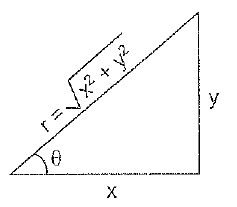
\includegraphics[scale=0.8]{pitagoras.png} \\
 \begin{equation}
  f(z) = u(r,\theta) + j v(r,\theta)
 \end{equation}
 La relación entre las coordenadas cartesianas y las coordenadas polares es: $x=r \cos(\theta)$ y $y=r \sen(\theta)$, $\theta = arctg(\dfrac{y}{x})$ 
 \end{multicols}
 Calcularemos las derivadas parciales de $u$ y $v$ con respecto a $x$ y $y$, para esto aplicaremos la regla de la cadena 
 \begin{center}
  $\displaystyle \left\{ 
  \begin{array}{lcr}
   \dfrac{\partial u}{\partial x} = \dfrac{\partial u}{\partial r} . \dfrac{\partial r}{\partial x} + \dfrac{\partial u}{\partial \theta} . \dfrac{\partial \theta}{\partial x} & (1)\\ \\
   \dfrac{\partial u}{\partial y} = \dfrac{\partial u}{\partial r} . \dfrac{\partial r}{\partial y} + \dfrac{\partial u}{\partial \theta} . \dfrac{\partial \theta}{\partial y} & (2)\\ \\
   \dfrac{\partial v}{\partial x} = \dfrac{\partial v}{\partial r} . \dfrac{\partial r}{\partial x} + \dfrac{\partial v}{\partial \theta} . \dfrac{\partial \theta}{\partial x} & (3)\\ \\
   \dfrac{\partial v}{\partial y} = \dfrac{\partial v}{\partial r} . \dfrac{\partial r}{\partial y} + \dfrac{\partial v}{\partial \theta} . \dfrac{\partial \theta}{\partial y} & (4)\\ \\ 
   \end{array}   
\right.$
 \end{center}
$r = \sqrt{x^2 + y^2} \Rightarrow \displaystyle \left\{ 
  \begin{array}{lcr}
   \dfrac{\partial r}{\partial x} = \dfrac{x}{\sqrt{x^2+y^2}} = \dfrac{x}{r} = \dfrac{r \cos(\theta)}{r}=\cos(\theta) \\
   \dfrac{\partial r}{\partial y} = \dfrac{y}{\sqrt{x^2+y^2}} = \dfrac{y}{r} = \dfrac{r \sen(\theta)}{r}=\sen(\theta) \\
   \end{array}   
\right.$ 
\\
$ \theta = arctg(\dfrac{y}{x}) \Rightarrow \displaystyle \left\{ 
  \begin{array}{lcr}
   \dfrac{\partial \theta}{\partial x} = \dfrac{-y}{x^2+y^2} = \dfrac{-y}{r^2} = \dfrac{-r \sen(\theta)}{r^2}=\dfrac{-1}{r} \sen(\theta) \\
   \dfrac{\partial \theta}{\partial y} = \dfrac{x}{x^2+y^2} = \dfrac{x}{r^2} = \dfrac{r \cos(\theta)}{r^2}=\dfrac{1}{r} \cos(\theta)
  \end{array}
\right.$ 
\\reemplazando en (1),(2),(3),(4), se tiene:
 \begin{center}
  $\displaystyle \left\{ 
  \begin{array}{lcr}
   \dfrac{\partial u}{\partial x} = \cos(\theta) \dfrac{\partial u}{\partial r} + \dfrac{1}{r} \sen(\theta) \dfrac{\partial u}{\partial \theta} & (5) \\ \\
   \dfrac{\partial u}{\partial y} = \sen(\theta)\dfrac{\partial u}{\partial r}  + \dfrac{1}{r} \sen(\theta) \dfrac{\partial u}{\partial \theta} & (6) \\ \\
   \dfrac{\partial v}{\partial x} = \cos(\theta) \dfrac{\partial v}{\partial r} + \dfrac{1}{r} \sen(\theta) \dfrac{\partial v}{\partial \theta} & (7) \\ \\
   \dfrac{\partial v}{\partial y} = \sen(\theta) \dfrac{\partial v}{\partial r} + \dfrac{1}{r} \cos(\theta) \dfrac{\partial v}{\partial \theta} & (8) \\ \\
   \end{array}   
\right.$
 \end{center}   
 pero por las ecuaciones de Cauchy-Riemann se tiene:
 $\displaystyle \dfrac{u}{x} - \dfrac{v}{y} = 0$ y $\displaystyle \dfrac{u}{y} + \dfrac{v}{x} = 0$  
 de las ecuaciones (5) y (8) se tiene:
 \begin{equation}
  \tag{9}
   (\dfrac{\partial u}{\partial r} - \dfrac{1}{r} \dfrac{\partial v}{\partial \theta}) \cos(\theta) - (\dfrac{1}{r} \dfrac{\partial u}{\partial \theta} +  \dfrac{\partial v}{\partial r}) \sen(\theta)=0 
 \end{equation}
 de las ecuaciones (6) y (7) se tiene: 
 \begin{equation}
  \tag{10}
  (\dfrac{1}{r} . \dfrac{\partial u}{\partial \theta} + \dfrac{\partial v}{\partial r}) \cos(\theta) - (\dfrac{\partial u}{\partial r} - \dfrac{1}{r} \dfrac{\partial v}{\partial \theta}) \sen(\theta) = 0 
 \end{equation}
 a las ecuaciones (9) y (10) multiplicamos por $cos(\theta)$ y $sen(\theta)$ respectivamente:
 \begin{equation}
  \tag{*}
  (\dfrac{\partial u}{\partial r} - \dfrac{1}{r} \dfrac{\partial v}{\partial \theta}) \cos^2(\theta) + (\dfrac{1}{r}\dfrac{\partial u}{\partial \theta} -  \dfrac{\partial v}{\partial r}) \sen(\theta) \cos(\theta) = 0 
 \end{equation}
 \begin{equation}
  \tag{**}
  (\dfrac{1}{r} . \dfrac{\partial u}{\partial \theta} + \dfrac{\partial v}{\partial r}) \cos(\theta). \sen(\theta) + (\dfrac{\partial u}{\partial r} - \dfrac{1}{r} \dfrac{\partial v}{\partial \theta}) \sen^2(\theta) = 0 
 \end{equation}
 ahora sumando (*) y (**) y se obtiene:
 \begin{center}
 $ (\dfrac{\partial u}{\partial r} - \dfrac{1}{r} \dfrac{\partial v}{\partial \theta})(\cos^2(\theta)) + \sen^2(\theta)) = 0 $
 \end{center}
de donde: $\dfrac{\partial u}{\partial r} - \dfrac{1}{r} \dfrac{\partial v}{\partial \theta} = 0$ \\
por lo tanto: \textbf{$\dfrac{\partial u}{\partial r} = \dfrac{1}{r}.\dfrac{\partial v}{\partial \theta}$} \\ \\
nuevamente a las ecuaciones (9) y (10) multiplicamos por $-\sen(\theta)$ y $\cos(\theta)$ respectivamente: 
\begin{equation}
 \tag{a}
 -(\dfrac{\partial u}{\partial r} - \dfrac{1}{r} \dfrac{\partial v}{\partial \theta}) \sen(\theta).\cos(\theta) +  (\dfrac{1}{r} \dfrac{\partial u}{\partial \theta} +  \dfrac{\partial v}{\partial r}) \sen^2(\theta)=0 
\end{equation}
\begin{equation}
  \tag{b}
  \dfrac{1}{r} . (\dfrac{\partial u}{\partial \theta}) \cos^2(\theta) + (\dfrac{\partial u}{\partial r} - \dfrac{1}{r} \dfrac{\partial v}{\partial \theta}) \sen(\theta) . \cos(\theta) = 0 
 \end{equation}
 al sumar (a) y (b) se obtiene:
 $(\dfrac{1}{r}.\dfrac{\partial u}{\partial \theta} + \dfrac{\partial v}{\partial r}) (\cos^2 (\theta) + \sen^2(\theta)) = 0 \Rightarrow \dfrac{1}{r}.\dfrac{\partial u}{\partial \theta} + \dfrac{\partial v}{\partial r}$ \\
 $\therefore \dfrac{\partial v}{\partial r}= - \dfrac{1}{r}.\dfrac{\partial u}{\partial \theta}$ \\ \\
 por lo tanto las ecuaciones de CAUCHY-RIEMANN en coordenadas polares son:
\begin{center}
 \textbf{$\dfrac{\partial u}{\partial r} = \dfrac{1}{r}.\dfrac{\partial v}{\partial \theta}$} y \textbf{$\dfrac{\partial v}{\partial r} = -\dfrac{1}{r}.\dfrac{\partial u}{\partial \theta}$}
\end{center}
\subsection{COORDENADAS CONJUGADAS}
El número complejo $z \in \mathbb{C}$ y su conjugado $\overline{z} \in \mathbb{C}$ , son determinadas en forma única por un par de coordenadas $(x,y)$ dadas por $z = x +jy$ , $\overline{z} = x -jy$ de donde $x = \dfrac{1}{2}(z+\overline{z})$ y $y = \dfrac{1}{2j}(z-\overline{z})$ entonces el par $(z,\overline{z})$ se llama "coordenadas conjugadas". \\
Las ecuaciones: $\displaystyle z = x +jy$ , $\displaystyle \overline{z} = x -jy$\\
\begin{center}
 $\displaystyle x =\dfrac{1}{2}(z+\overline{z})$ , $\displaystyle y = \dfrac{1}{2j}(z-\overline{z})$
\end{center}
nos permite transformar las coordenadas rectangualres $(x,y)$ a coordenadas conjugadas $\displaystyle (z,\overline{z})$   \\
\subsection{FUNCIONES ANALÍTICAS}
\textbf{a) DEFINICIÓN.- } Diremos que la función $f: D\subset C \rightarrow C$ es analítica en el punto $z_0 \in D$ , si $f$ está definida y es derivable en alguna vecindad de $z_0$, es decir "f" es analítica en $z_0$ si: $\exists V_\rho (z_0)$ tal que $f$ esta definida en $V_\rho (z_0)$ y $\displaystyle \exists$ $ f'(z_0)$ , $\forall z \in V_\rho (z_0)$
\begin{center}
 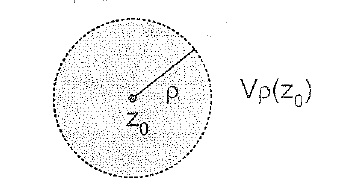
\includegraphics[scale=0.7]{analiticas.png}
\end{center}
\textbf{b) DEFINICIÓN.- } La función $f:D\subset \mathbb{C} \rightarrow \mathbb{C}$ es analítica en $D$, si $f$ es derivable $\forall z \in D$ \\
\textbf{OBSERVACIÓN.- }		A la función analítica también se le llama función regular u holomorfa\\
\textbf{OBSERVACIÓN.- }		La derivada de uan función analítica u holomorfa también analítica, de aquí es que una función analítica tiene derivadas de todos los ordenes\\
\textbf{c) DEFINICIÓN.- } Si la función $f:D\subset \mathbb{C} \rightarrow \mathbb{C}$ es analítica en todo $\mathbb{C}$, se le llama función entera \\
\textbf{a) FUNCIONES ARMÓNICAS.- }   \\
Si la función $f(z)=u(x,y) +jv(x,y)$ es analítica en $D$ entonces:
\begin{center}
 $\dfrac{\partial u(x,y)}{\partial x} = \dfrac{\partial v(x,y)}{\partial y} $	$\wedge$	$\dfrac{\partial u(x,y)} {\partial y} = -\dfrac{\partial v(x,y)}{\partial x}$ , $\forall (x,y) \in D$ \\
 $\dfrac{\partial^2 u(x,y)}{\partial x^2} = \dfrac{\partial^2 v(x,y)}{\partial x \partial y} $	$\wedge$	$\dfrac{\partial^2 u(x,y)}{\partial y^2} = -\dfrac{\partial^2 v(x,y)}{\partial y \partial x}$
\end{center}
 como $\dfrac{\partial^2 u(x,y)}{\partial x^2} = \dfrac{\partial^2 v(x,y)}{\partial x \partial y}$ , $\forall (x,y) \in D$ puesto que sus derivadas parciales son continuas, entonces:
 \begin{center}
  $\dfrac{\partial^2 u(x,y)}{\partial x^2} = \dfrac{\partial^2 u(x,y)}{\partial^2 y} = 0$ , $\forall (x,y) \in D$ 
 \end{center}
 $\displaystyle \left\{ 
  \begin{array}{lcr}
    \dfrac{\partial u(x,y)}{\partial x} = \dfrac{\partial v(x,y)}{\partial y} \\
    \dfrac{\partial u(x,y)} {\partial y} = -\dfrac{\partial v(x,y)}{\partial x}\\
   \end{array}   
\right.$ 
	$\Rightarrow$	 $\displaystyle \left\{ 
  \begin{array}{lcr}
    \dfrac{\partial^2 v(x,y)}{\partial y^2} = \dfrac{\partial^2 u(x,y)}{\partial y \partial x} \\
    \dfrac{\partial^2 v(x,y)}{\partial x^2} = -\dfrac{\partial^2 u(x,y)}{\partial x \partial y}\\
   \end{array}   
\right.$ , sumando \\
\begin{center}
 $\dfrac{\partial^2 v(x,y)}{\partial x^2} + \dfrac{\partial^2 v(x,y)}{\partial y^2} = 0 $ , $\forall (x,y) \in D$ \\
\end{center}  
 por lo tanto las partes real e imaginaria de una función compleja $f(z)=u(x,y) + jv(x,y)$ analíticas son soluciones de la ecuación de Laplace, donde:
 $\nabla^2 u = \dfrac{\partial^2 u}{\partial x^2} + \dfrac{\partial^2 u}{\partial y^2}$ \textbf{(Ecuación de Laplace de u)} \\
 $\nabla^2 v = \dfrac{\partial^2 v}{\partial x^2} + \dfrac{\partial^2 v}{\partial y^2}$ \textbf{(Ecuación de Laplace de v)} \\
Este caso se dice también que $u$ y $v$ son funciones armónicas, además $u$ y $v$ son un par de conjugadas armónicas una con respecto a la otra. \\
\textbf{OBSERVACIÓN.- } Las ecuaciones siguientes: \\
$\displaystyle \left\{ 
  \begin{array}{lcr}
    u_{xx} + u_{yy} = 0 \\
    v_{xx} + v_{yy} = 0 \\
   \end{array}   
\right.$ \\
se llaman ecuaciones de Laplace de dos variables que en Física se conoce con el nombre de ecuación de potencial\\
\subsection{DEFINICIÓN} Toda función $F(z)=u(x,y)+jv(x,y)$ que satisface las ecuaciones de Laplace se llaman "Funciones Armónicas" y $F(z)=u(x,y)+jv(x,y)$ es analítica, entonces $u$ y $v$ se llaman "conjugadas armónicas"

\end{document}
